% ==========================================================================
\section{Appendixes}
% ==========================================================================
\label{sec:appendixes}

    % ==========================================================================
    \subsection{ANSI Terminal colours}
    % ==========================================================================

    \begin{itemize}
        \item ANSI\_COLR\_BLK - Black
        \item ANSI\_COLR\_RED - Red
        \item ANSI\_COLR\_GRN - Green
        \item ANSI\_COLR\_YLW - Yellow
        \item ANSI\_COLR\_BLU - Blue
        \item ANSI\_COLR\_MGT - Magenta
        \item ANSI\_COLR\_CYA - Cyan
        \item ANSI\_COLR\_WHT - White
    \end{itemize}

    % ==========================================================================
    \subsection{VDP Composite colours}
    % ==========================================================================
    \label{sec:vdp_colours}

    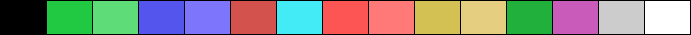
\includegraphics[scale=0.7]{images/TMS9918Apalette.png}

    \begin{itemize}
        \item VDP\_COLR\_TRNSP  (Transparent)   = \$00
        \item VDP\_COLR\_BLACK  (Black)         = \$01
        \item VDP\_COLR\_M\_GRN (Medium Green)  = \$02
        \item VDP\_COLR\_L\_GRN (Light Green)   = \$03
        \item VDP\_COLR\_D\_BLU (Dark Blue)     = \$04
        \item VDP\_COLR\_L\_BLU (Light Blue)    = \$05
        \item VDP\_COLR\_D\_RED (Dark Red)      = \$06
        \item VDP\_COLR\_CYAN   (Cyan)          = \$07
        \item VDP\_COLR\_M\_RED (Medium Red)    = \$08
        \item VDP\_COLR\_L\_RED (Light Red)     = \$09
        \item VDP\_COLR\_D\_YLW (Dark Yellow)   = \$0A
        \item VDP\_COLR\_L\_YLW (Light Yellow)  = \$0B
        \item VDP\_COLR\_D\_GRN (Dark Green)    = \$0C
        \item VDP\_COLR\_MGNTA  (Magenta)       = \$0D
        \item VDP\_COLR\_GREY   (Grey)          = \$0E
        \item VDP\_COLR\_WHITE  (White)         = \$0F
    \end{itemize}

    % ==========================================================================
    \subsection{VDP Screen resolutions}
    % ==========================================================================
    \label{sec:vdpscrmodes}


        % ==========================================================================
        \subsubsection{Mode 0: \textbf{Text Mode}}
        % ==========================================================================
        \begin{itemize}
            \item Screen is divided into 960 pattern positions each of which is
                capable of displaying a character. There are 40 characters in
                each row and 24 rows in total.
            \item Each character is 6 horizontal pixels by 8 vertical pixels.
            \item Each character can have 2 colours (Foreground and Background).
            \item Sprites cannot be used.
            \item Pattern Table:
            \begin{itemize}
                \item This table contains the character sets, for a maximum of
                    256 characters per set.
                \item Up to 7 different character sets can be held in the
                    \textbf{VRAM} at the same time. Each set MUST be located
                    starting at an \texttt{0x0800} boundary (i.e. 
                    \texttt{0x0000}, \texttt{0x1000}, \texttt{0x1800},
                    \texttt{0x2000}, \texttt{0x2800}, \texttt{0x3000} and
                    \texttt{0x3800}). Note that \texttt{0x0800} is not listed
                    because that address is used by the Name Table.
                \item Ideally, the patterns follow the ASCII table definitions
                    and order, so that the Name Table can be easily used to
                    display text by for example assigning the value \texttt{0x41}
                    to a byte in the Name Table to display the character
                    \textit{A}.
            \end{itemize}
            \item Name Table:
            \begin{itemize}
                \item Each entry in the table is 1 byte long and therefore can
                    specify one of 256 patterns (from \texttt{0x00} to
                    \texttt{0xFF}).
                \item Each entry represents a pattern position on the screen.
                    Position 0 is in the top left of the screen. Position 39 is
                    in the top right of the screen. The second row ranges from
                    40 to 79, and so on.
            \end{itemize}
        \end{itemize}

        % ==========================================================================
        \subsubsection{Mode 1: \textbf{Graphics I Mode}}
        % ==========================================================================
        \begin{itemize}
            \item Screen is divided into 768 blocks of 8x8 pixels each. There
                are 32 blocks in a row and 24 rows on the screen.
            \item Sprites can be used.
            \item Screen resolution is 256 by 192 pixels.
            \item Name Table:
            \begin{itemize}
                \item This table has 768 entries, one for each block on the screen.
                \item If the Pattern Table is loaded with with a full ASCII
                    character set, the entry of any ASCII value in the Name
                    Table will result in the corresponding character being
                    displayed on the screen.
            \end{itemize}
            \item Colour Table:
            \begin{itemize}
                \item This table has 32 entries, each entry defining 2 colours
                (Foreground and Background) out of 15 colours available, for a
                block of 8 characters. In other words, colours cannot be
                assigned independently to each character in the screen, but
                instead to groups of 8 consecutive characters.
            \end{itemize}
        \end{itemize}

        % ==========================================================================
        \subsubsection{Mode 2: \textbf{Graphics II Mode}}
        % ==========================================================================
        \begin{itemize}
            \item Screen is divided into 768 blocks of 8x8 pixels each. There
            are 32 blocks in a row and 24 rows on the screen.
            \item Sprites can be used.
            \item Screen resolution is 256 by 192 pixels.
            \item Name Table:
            \begin{itemize}
                \item This table is divided into three subtables of 256 each.
            \end{itemize}
            \item Colour Table:
            \begin{itemize}
                \item Each entry in the Colour Table is 8 bytes and each byte
                    defines the 2 colours (Foreground and Background) of each 
                    of the 8 rows of the character, from a total of 15 colours
                    plus transparent available.
            \end{itemize}
        \end{itemize}

        % ==========================================================================
        \subsubsection{Mode 3: \textbf{Multicolour Mode}}
        % ==========================================================================
        \begin{itemize}
            \item Screen is divided into 768 blocks of 2x2 squares. Each square
                is 4 pixels. There are 32 blocks in each row and 4 rows in each
                section. There are 6 sections, for a total of 24 rows on the
                screen.
            \item Blocks are arranged in columns with 4 blocks in each column.
            \item Columns are arranged in sections, with 32 columns in each
                section.
            \item There are a total of 6 sections on the screen.
            \item In summary:
            \begin{itemize}
                \item 32 columns * 6 sections = 192 columns
                \item 192 columns * 4 blocks = 768 blocks
            \end{itemize}
            \item No characters for text can be used.
            \item Sprites can be used.
            \item The Colour Table is not used. Instead, the colour of the boxes
            are defined in the Pattern Table.
            \item Pattern Table:
            \begin{itemize}
                \item Each entry in the table is 8 bytes, but only 2 bytes are
                        used to define the colours of the 4 boxes that make up
                        a character.
            \end{itemize}
        \end{itemize}

        % ==========================================================================
        \subsubsection{Mode 4: \textbf{Graphics II Mode Bitmapped}}
        % ==========================================================================
        \begin{itemize}
            \item Same as Mode 2, but screen is bitmapped for addressing every
                pixel individually.
            \item Pixels cannot have colours assigned individually. Instead
                colour is assigned by a byte, where each bit tells if the pixel
                is visible (bit=1) or not (bit=0). Therefore, pixels are grouped
                in groups of 8. For example, \texttt{0x4F} (0100 1111) will set
                pixels 0, 1, 2, 3 and 6 as visible, and pixels 4, 5, and 7 not
                visible. Pixels that are visible will have dark blue colour
                (\texttt{0x04}) over white background (\texttt{0x0F}).
        \end{itemize}

    % ==========================================================================
    \subsection{VDP Limitations}
    % ==========================================================================
    \label{subsec:vdp_limitations}

    The maximum resolutions are: 240x192 pixels in Text Mode, 256x192 pixels in
    Graphics Modes (I, II, II Bit-mapped), and 512x384 in Multicolour Mode.

    The maximum number of colours is 15 plus a transparent colour.

    In Graphics I Mode, each entry in the Colour Table defines the colour for
    a group of eight patterns. Hence, individual character colouring is not
    possible.

    In Graphics II Bit-mapped Mode, individual pixels can be addressed but
    individual colours cannot. Therefore it is not possible to assign different
    colours for each pixel.

    Bug?: After some tests, and confirmed with some information found on the
    Internet, reading continuously the Status Register can lead to miss the flag.
    This happens when the register is read and the VDP is about to set it,
    because as specified in the \textit{Video Display Processors Programmer's
    Guide}\cite{ti1}, \textit{the Status Register is reset after it's read}.
    Therefore, the subroutine implemented in dzOS for waiting for the VBLANK
    (\textit{BIOS\_VDP\_VBLANK\_WAIT}) that initially was reading the
    \textbf{VDP}'s Status Register and looping until the MSB changed to 1, has
    been changed to instead check for a change on the
    \hyperref[subsec:jiffy_counter]{Jiffy Counter}.

    % ==========================================================================
    \subsubsection{Sprites}
    % ==========================================================================

    A maximum of 32 sprites can be shown on the screen, of sizes either 8x8 or
    16x16 pixels. Though sprites can be magnified, thus showing as 16x16 or
    32x32 respectively.

    The location of a sprite is defined by the top left-hand corner of the
    sprite pattern.

    When more than one sprite is located at the same screen coordinate, the
    sprite on the higher priority plane will be shown.

    A maximum of 4 sprites can be displayed on the same horizontal line. If this
    rule is violated, the four highest priority sprites on the line are
    displayed normally, but the fifth and subsequent sprites are not displayed.

    The \textit{Coincidence Flag} (collision dectection) only indicates that
    any two sprites have overlapping bits, but it does not tell which sprites
    are. This must be calculated programatically.

    % ==========================================================================
    \subsection{Jiffy Counter}
    % ==========================================================================
    \label{subsec:jiffy_counter}

    A \textit{Jiffy} is the time between two ticks of the system timer interrupt.
    On the dastaZ80, this timer is generated by the TMS9918A (\textbf{VDP}) at
    roughly each 1/60th second.\\

    The counter is made of 3 bytes. Byte 1 is incremented in each \textbf{VDP}
    interrupt. Once it rolls over to zero (256 increments), the byte 2 is
    incremented. Once the byte 2 rolls over, the byte 3 is incremented. Once the
    three bytes together (24-bit) reach the value \texttt{0x4F1A00}, the three
    bytes are initialised to zero.

    \texttt{0x4F1A00} (5,184,000 in decimal) is the number of jiffies in 24
    hours: 24 hours x 60 minutes in an hour x 60 seconds in a minute x 60
    jiffies in a second.

    \textbf{IMPORTANT}: This counter MUST not be interpreted as an accurate
    clock, because when transferring data to the \textbf{VRAM} the OS disables
    the \hyperref[sec:nmi]{NMI}\footnote{It is also highly recommended that in
    your programs you also disable the \hyperref[sec:nmi]{NMI} when copying
    large amounts of data. Otherwise, the process will be interrupted 60 times
    per second, and therefore slow it down.}, and therefore the counter stops
    for a while.

    % ==========================================================================
    \subsection{OS Boot Sequence}
    % ==========================================================================
    After power on or after pressing the \textbf{RESET} button:

    \begin{itemize}
        \item \textbf{Bootstrap}
        \begin{itemize}
            \item Copy contents of the ROM into High RAM (\texttt{0x8000} - \texttt{0xFFFF}).
            \item Disable ROM chip and enable Low RAM (\texttt{0x0000} - \texttt{0x7FFF}).
            Therefore, all \textbf{MEMORY} is RAM from now on.
            \item Copy the copy of ROM inm High RAM to Low RAM. Bootstrap code is not copied.
            \item Transfer control to BIOS (\texttt{jp F\_BIOS\_SERIAL\_INIT}).
        \end{itemize}
        \item \textbf{Initialise SIO/2} (\texttt{F\_BIOS\_SERIAL\_INIT})
        \begin{itemize}
            \item Initialise SIO/2.
            \begin{itemize}
                \item Set Channel A as 115,000 bps, 8N1, Interrupt in all 
                received characters.
                \item Set Channel B as 115,000 bps, 8N1, Interrupt in all 
                received characters.
                \item Set Interrupt Vector to \texttt{0x60}.
            \end{itemize}
            \item Set CPU to Interrupt Mode 2.
            \item \texttt{jp F\_BIOS\_WBOOT}
        \end{itemize}
        \item \textbf{BIOS Boot} (\texttt{F\_BIOS\_WBOOT})
        \begin{itemize}
            \item Enable NMI (VDP) interrupts.
            \item Set NMI jump address to default value.
            \item Transfer control to Kernel (\texttt{jp F\_KRN\_START}).
        \end{itemize}
        \item \textbf{Kernel Boot} (\texttt{F\_KRN\_START})
        \begin{itemize}
            \item Display dzOS welcome message.
            \item Display dzOS release version.
            \item Display BIOS version.
            \item Display Kernel version.
            \item Display available \textbf{RAM}.
            \item Initialise \textbf{VDP}.
            \begin{itemize}
                \item Test write/read \textbf{VRAM}.
                \item Set \textbf{Low Resolution Display} as \textit{Graphics II
                Bit-mapped Mode}.
                \item Show dastaZ80 Logo in the \textbf{Low Resolution Display}.
            \end{itemize}
            \item Initialise \textbf{PSG}.
            \begin{itemize}
                \item Set Noise OFF, Audio OFF, I/O Port as Output.
                \item Make a beep.
            \end{itemize}
            \item Initialise \textbf{FDD}.
            \item Initialise \textbf{SD Card}.
            \begin{itemize}
                \item Detect \textbf{SD Card}.
                \item Display number of available Disk Image Files.
                \item Display disk unit and name of each Disk Image File.
            \end{itemize}
            \item Initialise \textbf{Real-Time Clock (RTC)}.
            \begin{itemize}
                \item Display current date and time.
                \item Display \textbf{RTC}'s battery status.
            \end{itemize}
            \item Initialise \hyperref[sec:ram_memmap]{SYSVARS}.
            \begin{itemize}
                \item Set show deleted files with \textit{cat} command as OFF.
                \item Set default File Type as 0 (USR = User defined).
                \item Set default loadsave address to \texttt{0x0000} (i.e. will
                save/load starting from \hyperref[subsec:memmap:ram]{Free RAM}
                (\texttt{0x4420})).
            \end{itemize}
            \item Set default \textbf{DISK} as 1 (i.e. first Disk Image File in
            the \textbf{SD card}).
            \item Transfer control to Command-line Interpreter (CLI) (\texttt{jp F\_CLI\_START}).
        \end{itemize}
        \item \textbf{CLI} (\texttt{F\_CLI\_START})
        \begin{itemize}
            \item Display CLI version.
            \item Clear command buffers
            \item Display prompt ($>$).
            \item Read command entered by user.
            \item Parse command.
            \item Execute corresponding subroutine.
            \item Loop back to Display prompt.
        \end{itemize}
    \end{itemize}

    % ==========================================================================
    \subsection{dzOS Programming Style}
    % ==========================================================================

    When writting dzOS and software for dzOS, the following style has been
    followed:

    \begin{itemize}
        \item All CPU registers are witten in uppercase (e.g. \textit{A},
        \textit{BC}, \textit{HL}, \textit{IX}, \textit{SP}).
        \item All CPU flags are witten in lowercase (e.g. \textit{z},
        \textit{nz}, \textit{c}, \textit{nc}, \textit{m}, \textit{p}).
        \item All assembly mnemonics are written in lowercase (e.g. 
        \textit{ld A,0}).
        \item Labels for subroutines that will be public (i.e. called via a
        Jumpblock) are written in uppercase.
        \item Labels are written in a line, with no mnemonics.
        \item Public subroutines contain comments specifying:
        \begin{itemize}
            \item Short description.
            \item Input CPU registers or variables (\hyperref[sec:ram_memmap]{SYSVARS}).
            \item Output CPU registers or variables (\hyperref[sec:ram_memmap]{SYSVARS}).
        \end{itemize}
        \item All hexadecimal values are written with a dollar sign as prefix.
        \item Tabulation (Tabs) are written as 4 spaces.
        \item Mnemonics start after 2 tabs (8 spaces).
        \item When possible, comments are written in column 41. Otherwise in
        next closest Tab.
        \item Source code is heavily commented. Mostly on each line.
        \item \textit{The Telemark Assembler} (TASM) specific:
        \begin{itemize}
            \item \textit{.BYTE} is used instead of \textit{.DB}
            \item \textit{.WORD} is used instead of \textit{.DW}
        \end{itemize}
    \end{itemize}

    % ==========================================================================
    \subsection{How a BASIC program is stored in RAM}
    % ==========================================================================

    When a user enters a program line (e.g. \texttt{10 PRINT "HELLO WORLD"}),
    BASIC must store it somewhere in \textbf{RAM} so that it can be retrieved
    later when for example the user wants to run, list or save the program.

    If all bytes would have to be stored, our example above would require 20
    bytes for the text code (including space between line number and PRINT),
    plus at least 2 bytes more for the line counter.

    The authors of MS BASIC cleverly decided that instead of storing the BASIC
    statements as ASCII characters, needing one byte per character, it would be
    enough to give each statement a unique identifier of one byte and instead
    store that byte. This unique identifier is commonly know as \textit{token}.

    For example, the \texttt{PRINT} statement has the token \texttt{0x9E}, so
    instead of needing 5 bytes to store each letter of the word \textit{PRINT},
    BASIC just needs 1 byte. It has saved 4 bytes. Imagine how much can save in
    a program with hundreds or even thousand of lines.

    So how it's a program stored in RAM, now that we know BASIC will use tokens
    for each reserved word instead of storing each character of the word?

    Lets take our previous example: \texttt{10 PRINT "HELLO WORLD"}

    Assuming the program is stored at address \texttt{0x80F9}, it will be stored
    as:

    \texttt{
    \resizebox{12cm}{!}{
        \begin{tabular}{l l l l l l l l l l l l l l l l l}
            80F9: & 00 & 0E & 81 & 0A & 00 & 9E & 20 & 22 & 48 & 45 & 4C & 4C & 4F & 20 & 57 & 4F\\
            810F: & 52 & 4C & 44 & 22 & 00 & 00 & 00\\
        \end{tabular}
    }}

    where:

    \begin{itemize}
        \item \texttt{00}: flag indicates start of program.
        \item \texttt{0E 81}: address to the next line in memory. In this
        example equals to end of program as there are no more lines.
        \item \texttt{0A 00}: line 10 in little-endian.
        \item \texttt{9E}: token for PRINT.
        \item \texttt{20}: space character.
        \item \texttt{22}: double quote (") character.
        \item \texttt{48 45 4C 4C 4F}: characters for HELLO.
        \item \texttt{20}: space character.
        \item \texttt{57 4F 52 4C 44}: characters for WORLD.
        \item \texttt{22}: double quote (") character.
        \item \texttt{00}: flag indicates end of line.
        \item \texttt{00 00}: flag indicates end of program.
    \end{itemize}

    Now it's easy to understand why some programs published in books and
    magazines skip some of the blank spaces, and write \texttt{FOR I=0 TO 10}
    instead as \texttt{FORI=0TO10}. It saves 3 bytes in memory by not having to
    store the space characters \texttt{0x20}. It also increases a bit the
    running speed, as the BASIC interpreter doesn't have to parse and interpret
    each of the spaces.

    % ==========================================================================
    \subsection{How a BASIC program is stored in DISK}
    % ==========================================================================

    \begin{itemize}
        \item 2 bytes: Address of PROGND (End of program). Start of variables
            area. This is where the variables are stored.
        \item 2 bytes: Address of VAREND (End of variables). Start of arrays
            area. This is where the arrays are stored.
        \item 2 bytes: Address of ARREND (End of arrays). This contains the
            address of the byte after last array.
        \item 2 bytes: Address of NXTDAT (Next DATA item). This contains the
            address of the next item of DATA to be READ.
        \item 2 bytes: Address of FNRGNM (FN argument name). This contains the
            name of the argument for the current FN function.
        \item 4 bytes: Address of FNARG (FN function argument). This is the
            floating point value of the current FN function's argument.
        \item 4 bytes: Address of FPREG (Floating point register). This is a
            floating point number for the current value.
        \item 1 byte: Address of SGNRES (Sign of result). This contains the sign
            of the result for multiplication.
        \item 13 bytes: Address of PBUFF (Number print buffer). When a floating
            point number has to be converted into ASCII for PRINT or STR\$ the
            ASCII number is built up in this buffer.
        \item 3 bytes: Address of NULVAL (Multiply value). This contains the
            24-bit multiplier.
        \item n bytes: tokenised BASIC program.
    \end{itemize}

    % ==========================================================================
    \subsection{How a BASIC floating point number is stored in RAM}
    % ==========================================================================

    Floating point is arithmetic that represents subsets of real numbers using
    an integer with a fixed precision, called the significand, scaled by an
    integer exponent of a fixed base.

    To store floating point numbers in MS BASIC, Microsoft introduced the
    \textit{Microsoft Binary Format} (MBF) in the very first version of MS BASIC
    (then called \textit{Altair BASIC}) in 1975.

    MBF single-precision format uses 4 bytes (32 bits):
    
    \begin{itemize}
        \item 1-bit sign (0=positive, 1=negative)
        \item 23-bit mantissa of the significand
        \item 8-bit base-2 exponent. Encoded with a bias of 128, so that
            negative exponents (-127 to -1) are reprsented by 1 to 127, and
            positive exponents (0 to 127) are represented by 128 to 255.
        \item Less significant 8 bits are unused
    \end{itemize}
